\documentclass{standalone}
\usepackage{tikz}
\usetikzlibrary{patterns, positioning}

\begin{document}
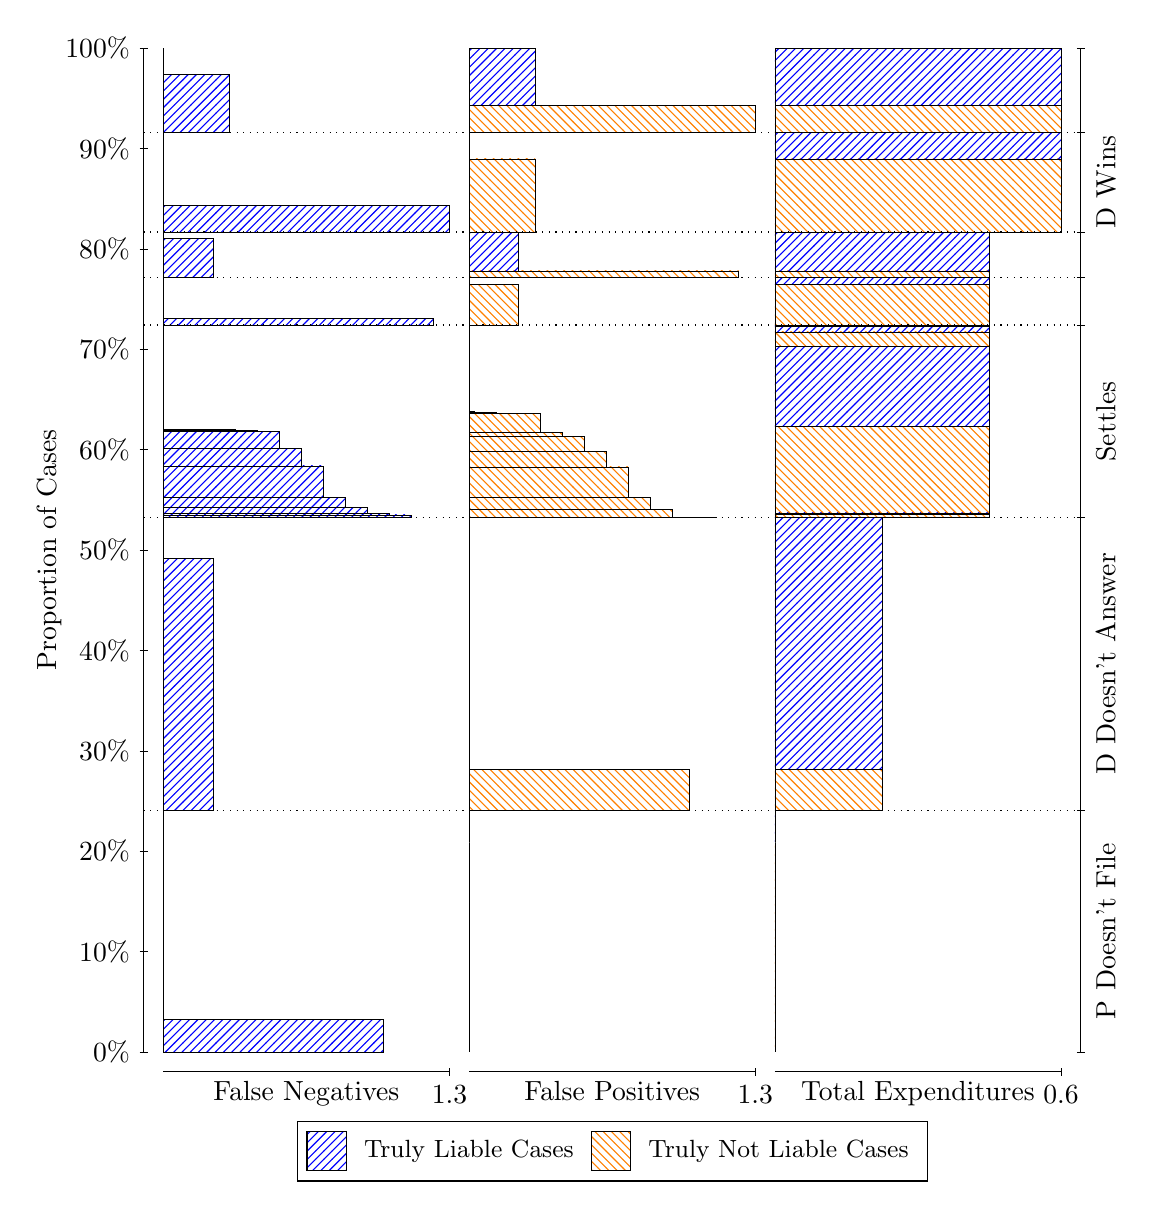
\begin{tikzpicture}
\draw[black, very thin] (1.5,1.75) -- (1.5,14.5);
\node[rotate=90, anchor=center] at (0.3, 8.125) {Proportion of Cases};
\draw[black, very thin] (1.45,1.75) -- (1.55,1.75);
\node[anchor=east] at (1.45, 1.75) {0\%};
\draw[black, very thin] (1.45,3.025) -- (1.55,3.025);
\node[anchor=east] at (1.45, 3.025) {10\%};
\draw[black, very thin] (1.45,4.3) -- (1.55,4.3);
\node[anchor=east] at (1.45, 4.3) {20\%};
\draw[black, very thin] (1.45,5.575) -- (1.55,5.575);
\node[anchor=east] at (1.45, 5.575) {30\%};
\draw[black, very thin] (1.45,6.85) -- (1.55,6.85);
\node[anchor=east] at (1.45, 6.85) {40\%};
\draw[black, very thin] (1.45,8.125) -- (1.55,8.125);
\node[anchor=east] at (1.45, 8.125) {50\%};
\draw[black, very thin] (1.45,9.4) -- (1.55,9.4);
\node[anchor=east] at (1.45, 9.4) {60\%};
\draw[black, very thin] (1.45,10.675) -- (1.55,10.675);
\node[anchor=east] at (1.45, 10.675) {70\%};
\draw[black, very thin] (1.45,11.95) -- (1.55,11.95);
\node[anchor=east] at (1.45, 11.95) {80\%};
\draw[black, very thin] (1.45,13.225) -- (1.55,13.225);
\node[anchor=east] at (1.45, 13.225) {90\%};
\draw[black, very thin] (1.45,14.5) -- (1.55,14.5);
\node[anchor=east] at (1.45, 14.5) {100\%};

\draw[black, very thin] (13.4,1.75) -- (13.4,14.5);
\draw[black, very thin] (13.35,1.75) -- (13.45,1.75);
\node[anchor=west] at (13.35, 1.75) {};
\draw[black, very thin] (13.35,4.8194) -- (13.45,4.8194);
\node[anchor=west] at (13.35, 4.8194) {};
\draw[black, very thin] (13.35,8.536) -- (13.45,8.536);
\node[anchor=west] at (13.35, 8.536) {};
\draw[black, very thin] (13.35,10.982) -- (13.45,10.982);
\node[anchor=west] at (13.35, 10.982) {};
\draw[black, very thin] (13.35,11.588) -- (13.45,11.588);
\node[anchor=west] at (13.35, 11.588) {};
\draw[black, very thin] (13.35,12.163) -- (13.45,12.163);
\node[anchor=west] at (13.35, 12.163) {};
\draw[black, very thin] (13.35,13.432) -- (13.45,13.432);
\node[anchor=west] at (13.35, 13.432) {};
\draw[black, very thin] (13.35,14.5) -- (13.45,14.5);
\node[anchor=west] at (13.35, 14.5) {};

\draw[black, very thin, pattern color=blue, pattern=north east lines] (1.75,1.75) rectangle (4.5449,2.1604);
\draw[black, very thin, pattern color=orange, pattern=north west lines] (1.75,2.1604) rectangle (1.75,4.8194);
\draw[black, very thin, pattern color=blue, pattern=north east lines] (1.75,4.8194) rectangle (2.3788,8.0164);
\draw[black, very thin, pattern color=orange, pattern=north west lines] (1.75,8.0164) rectangle (1.75,8.536);
\draw[black, very thin, pattern color=blue, pattern=north east lines] (1.75,8.536) rectangle (4.8942,8.5697);
\draw[black, very thin, pattern color=blue, pattern=north east lines] (1.75,8.5697) rectangle (4.6147,8.5851);
\draw[black, very thin, pattern color=blue, pattern=north east lines] (1.75,8.5851) rectangle (4.3353,8.6618);
\draw[black, very thin, pattern color=blue, pattern=north east lines] (1.75,8.6618) rectangle (4.0558,8.7967);
\draw[black, very thin, pattern color=blue, pattern=north east lines] (1.75,8.7967) rectangle (3.7763,9.1925);
\draw[black, very thin, pattern color=blue, pattern=north east lines] (1.75,9.1925) rectangle (3.4968,9.414);
\draw[black, very thin, pattern color=blue, pattern=north east lines] (1.75,9.414) rectangle (3.2173,9.6333);
\draw[black, very thin, pattern color=blue, pattern=north east lines] (1.75,9.6333) rectangle (2.9378,9.6423);
\draw[black, very thin, pattern color=blue, pattern=north east lines] (1.75,9.6423) rectangle (2.6583,9.657);
\draw[black, very thin, pattern color=orange, pattern=north west lines] (1.75,9.657) rectangle (1.75,10.982);
\draw[black, very thin, pattern color=blue, pattern=north east lines] (1.75,10.982) rectangle (5.1737,11.068);
\draw[black, very thin, pattern color=orange, pattern=north west lines] (1.75,11.068) rectangle (1.75,11.588);
\draw[black, very thin, pattern color=blue, pattern=north east lines] (1.75,11.588) rectangle (2.3788,12.08);
\draw[black, very thin, pattern color=orange, pattern=north west lines] (1.75,12.08) rectangle (1.75,12.163);
\draw[black, very thin, pattern color=blue, pattern=north east lines] (1.75,12.163) rectangle (5.3833,12.502);
\draw[black, very thin, pattern color=orange, pattern=north west lines] (1.75,12.502) rectangle (1.75,13.432);
\draw[black, very thin, pattern color=blue, pattern=north east lines] (1.75,13.432) rectangle (2.5885,14.162);
\draw[black, very thin, pattern color=orange, pattern=north west lines] (1.75,14.162) rectangle (1.75,14.5);
\draw[black, very thin, pattern color=orange, pattern=north west lines] (5.6333,1.75) rectangle (5.6333,4.409);
\draw[black, very thin, pattern color=blue, pattern=north east lines] (5.6333,4.409) rectangle (5.6333,4.8194);
\draw[black, very thin, pattern color=orange, pattern=north west lines] (5.6333,4.8194) rectangle (8.4282,5.339);
\draw[black, very thin, pattern color=blue, pattern=north east lines] (5.6333,5.339) rectangle (5.6333,8.536);
\draw[black, very thin, pattern color=orange, pattern=north west lines] (5.6333,8.536) rectangle (8.7776,8.538);
\draw[black, very thin, pattern color=orange, pattern=north west lines] (5.6333,8.538) rectangle (8.4981,8.5402);
\draw[black, very thin, pattern color=orange, pattern=north west lines] (5.6333,8.5402) rectangle (8.2186,8.64);
\draw[black, very thin, pattern color=orange, pattern=north west lines] (5.6333,8.64) rectangle (7.9391,8.7968);
\draw[black, very thin, pattern color=orange, pattern=north west lines] (5.6333,8.7968) rectangle (7.6596,9.1807);
\draw[black, very thin, pattern color=orange, pattern=north west lines] (5.6333,9.1807) rectangle (7.3801,9.3807);
\draw[black, very thin, pattern color=orange, pattern=north west lines] (5.6333,9.3807) rectangle (7.1006,9.5643);
\draw[black, very thin, pattern color=orange, pattern=north west lines] (5.6333,9.5643) rectangle (6.8212,9.6221);
\draw[black, very thin, pattern color=orange, pattern=north west lines] (5.6333,9.6221) rectangle (6.5417,9.861);
\draw[black, very thin, pattern color=blue, pattern=north east lines] (5.6333,9.861) rectangle (5.9827,9.8757);
\draw[black, very thin, pattern color=blue, pattern=north east lines] (5.6333,9.8757) rectangle (5.7032,9.8847);
\draw[black, very thin, pattern color=blue, pattern=north east lines] (5.6333,9.8847) rectangle (5.6333,10.982);
\draw[black, very thin, pattern color=orange, pattern=north west lines] (5.6333,10.982) rectangle (6.2622,11.502);
\draw[black, very thin, pattern color=blue, pattern=north east lines] (5.6333,11.502) rectangle (5.6333,11.588);
\draw[black, very thin, pattern color=orange, pattern=north west lines] (5.6333,11.588) rectangle (9.0571,11.671);
\draw[black, very thin, pattern color=blue, pattern=north east lines] (5.6333,11.671) rectangle (6.2622,12.163);
\draw[black, very thin, pattern color=orange, pattern=north west lines] (5.6333,12.163) rectangle (6.4718,13.093);
\draw[black, very thin, pattern color=blue, pattern=north east lines] (5.6333,13.093) rectangle (5.6333,13.432);
\draw[black, very thin, pattern color=orange, pattern=north west lines] (5.6333,13.432) rectangle (9.2667,13.771);
\draw[black, very thin, pattern color=blue, pattern=north east lines] (5.6333,13.771) rectangle (6.4718,14.5);
\draw[black, very thin, pattern color=orange, pattern=north west lines] (9.5167,1.75) rectangle (9.5167,4.409);
\draw[black, very thin, pattern color=blue, pattern=north east lines] (9.5167,4.409) rectangle (9.5167,4.8194);
\draw[black, very thin, pattern color=orange, pattern=north west lines] (9.5167,4.8194) rectangle (10.879,5.339);
\draw[black, very thin, pattern color=blue, pattern=north east lines] (9.5167,5.339) rectangle (10.879,8.536);
\draw[black, very thin, pattern color=orange, pattern=north west lines] (9.5167,8.536) rectangle (12.242,8.5745);
\draw[black, very thin, pattern color=blue, pattern=north east lines] (9.5167,8.5745) rectangle (12.242,8.595);
\draw[black, very thin, pattern color=orange, pattern=north west lines] (9.5167,8.595) rectangle (12.242,9.6956);
\draw[black, very thin, pattern color=blue, pattern=north east lines] (9.5167,9.6956) rectangle (12.242,10.711);
\draw[black, very thin, pattern color=orange, pattern=north west lines] (9.5167,10.711) rectangle (12.242,10.894);
\draw[black, very thin, pattern color=blue, pattern=north east lines] (9.5167,10.894) rectangle (12.242,10.971);
\draw[black, very thin, pattern color=orange, pattern=north west lines] (9.5167,10.971) rectangle (12.242,10.973);
\draw[black, very thin, pattern color=blue, pattern=north east lines] (9.5167,10.973) rectangle (12.242,10.982);
\draw[black, very thin, pattern color=orange, pattern=north west lines] (9.5167,10.982) rectangle (12.242,11.502);
\draw[black, very thin, pattern color=blue, pattern=north east lines] (9.5167,11.502) rectangle (12.242,11.588);
\draw[black, very thin, pattern color=orange, pattern=north west lines] (9.5167,11.588) rectangle (12.242,11.671);
\draw[black, very thin, pattern color=blue, pattern=north east lines] (9.5167,11.671) rectangle (12.242,12.163);
\draw[black, very thin, pattern color=orange, pattern=north west lines] (9.5167,12.163) rectangle (13.15,13.093);
\draw[black, very thin, pattern color=blue, pattern=north east lines] (9.5167,13.093) rectangle (13.15,13.432);
\draw[black, very thin, pattern color=orange, pattern=north west lines] (9.5167,13.432) rectangle (13.15,13.771);
\draw[black, very thin, pattern color=blue, pattern=north east lines] (9.5167,13.771) rectangle (13.15,14.5);
\draw[black, dotted] (1.5,4.8194) -- (13.4,4.8194);
\draw[black, dotted] (1.5,8.536) -- (13.4,8.536);
\draw[black, dotted] (1.5,10.982) -- (13.4,10.982);
\draw[black, dotted] (1.5,11.588) -- (13.4,11.588);
\draw[black, dotted] (1.5,12.163) -- (13.4,12.163);
\draw[black, dotted] (1.5,13.432) -- (13.4,13.432);
\draw[black, very thin] (1.75,1.5) -- (5.3833,1.5);
\node[anchor=north] at (3.5667, 1.5) {False Negatives};
\draw[black, very thin] (5.3833,1.45) -- (5.3833,1.55);
\node[anchor=north] at (5.3833, 1.45) {1.3};

\draw[black, very thin] (5.6333,1.5) -- (9.2667,1.5);
\node[anchor=north] at (7.45, 1.5) {False Positives};
\draw[black, very thin] (9.2667,1.45) -- (9.2667,1.55);
\node[anchor=north] at (9.2667, 1.45) {1.3};

\draw[black, very thin] (9.5167,1.5) -- (13.15,1.5);
\node[anchor=north] at (11.333, 1.5) {Total Expenditures};
\draw[black, very thin] (13.15,1.45) -- (13.15,1.55);
\node[anchor=north] at (13.15, 1.45) {0.6};

\node[black, centered, rotate=90] at (13.72, 3.2847) {P Doesn't File};
\node[black, centered, rotate=90] at (13.72, 6.6777) {D Doesn't Answer};
\node[black, centered, rotate=90] at (13.72, 9.759) {Settles};


\node[black, centered, rotate=90] at (13.72, 12.798) {D Wins};


\draw (7.449999999999999,1.5) node[draw=none] (baseCoordinate) {};
\begin{scope}[align=center]
        \matrix[scale=0.5, draw=black, below=0.5cm of baseCoordinate, nodes={draw}, column sep=0.1cm]{
            \node[rectangle, draw, minimum width=0.5cm, minimum height=0.5cm, pattern=north east lines, pattern color=blue] {}; &
            \node[draw=none, font=\small] (B) {Truly Liable Cases}; &
            \node[rectangle, draw, minimum width=0.5cm, minimum height=0.5cm, pattern=north west lines, pattern color=orange] {}; &
            \node[draw=none, font=\small] (B) {Truly Not Liable Cases}; \\
            };
\end{scope}

\end{tikzpicture}
\end{document}